\documentclass[tikz,svgnames,border={5 5}]{standalone}

\usepackage{mathtools}

\usetikzlibrary{positioning,arrows,fit}

\renewcommand\vec[1]{\boldsymbol{#1}}

\begin{document}
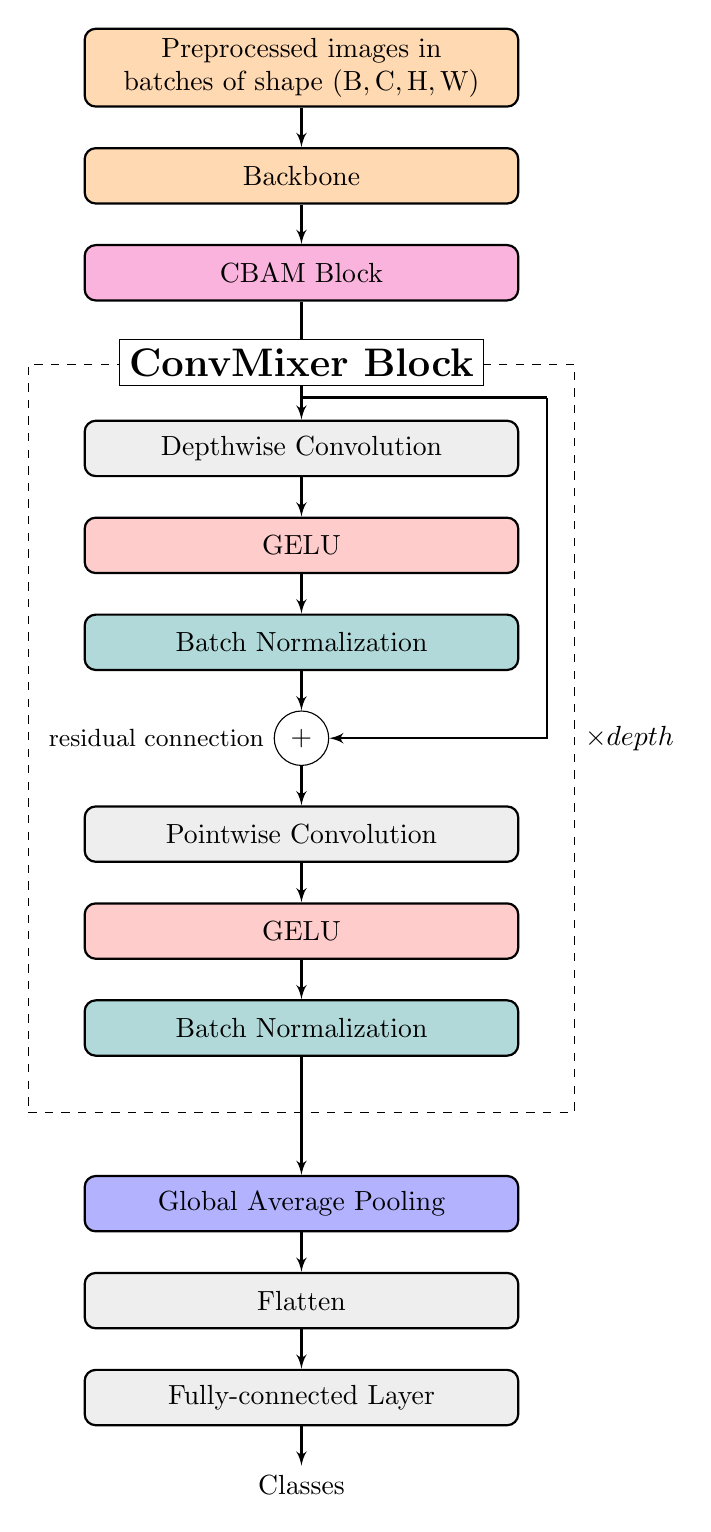
\begin{tikzpicture}[
    box/.style={rectangle,draw,fill=DarkGray!20,node distance=1cm,text width=15em,text centered,rounded corners,minimum height=2em,thick},
    arrow/.style={draw,-latex',thick},
  ]
  \node [box] (depthwise_conv) {Depthwise Convolution};
  \node [box,fill=red!20,below=0.5 of depthwise_conv] (activation1) {GELU};
  \node [box,fill=teal!30,below=0.5 of activation1] (norm1) {Batch Normalization};
  \node [circle,draw,below=0.5 of norm1] (residual) {+};
  \node [left=0 of residual] (residual text) {\small residual connection};
  \node [box,below=0.5 of residual] (pointwise_conv) {Pointwise Convolution};
  \node [box,fill=red!20,below=0.5 of pointwise_conv] (activation2) {GELU};
  \node [box,fill=teal!30,below=0.5 of activation2] (norm2) {Batch Normalization};

  \path
  (depthwise_conv.north west) ++(-1em,1em) coordinate (depthwise_conv fit)
  (norm2.south east) ++(1em,-1em) coordinate (norm2 fit)
  (depthwise_conv.north east) ++(1em,0.8em) coordinate (input fit)
  (depthwise_conv.south east) ++(1em,-9em) coordinate (residual fit);

  \node [box,above=1.5 of depthwise_conv, fill=magenta!30] (cbam) {CBAM Block};
  \node [box,above=0.5 of cbam, fill=orange!30] (backbone) {Backbone};
  \node [box,above=0.5 of backbone, fill=orange!30] (initial) {Preprocessed images in batches of shape $\mathrm{(B,C,H,W)}$};
  \node [box,below=1.5 of norm2, fill=blue!30] (pooling) {Global Average Pooling};
  \node [box,below=0.5 of pooling] (flatten) {Flatten};
  \node [box,below=0.5 of flatten] (fc) {Fully-connected Layer};
  \node [below=0.5 of fc] (classes) {Classes};

  \path [arrow] (initial) -- (backbone);
  \path [arrow] (backbone) -- (cbam);
  \path [arrow] (cbam) -- (depthwise_conv);
  \path [arrow] (depthwise_conv) -- (activation1);
  \path [arrow] (activation1) -- (norm1);
  \path [arrow] (norm1) -- (residual);
  \path [arrow] (residual) -- (pointwise_conv);
  \path [arrow] (pointwise_conv) -- (activation2);
  \path [arrow] (activation2) -- (norm2);

  \node [rectangle,draw,dashed,inner sep=1em,fit=(depthwise_conv fit) (norm2 fit)] (enclosure) {};
  \node [right=0 of enclosure] (depth) {$\times depth$};
  \node [above=-0.8em of enclosure,anchor=south,draw,outer sep=0pt,fill=white] (enclosure label) {\Large\textbf{ConvMixer Block}};

  \path [arrow] (norm2) -- (pooling);
  \path [arrow] (pooling) -- (flatten);
  \path [arrow] (flatten) -- (fc);
  \path [arrow] (fc) -- (classes);
  \path [draw,thick] (depthwise_conv.north) ++(0em,0.8em) -- (input fit); 
  \path [draw,thick] (residual fit) -- (input fit);
  \draw [arrow] (residual fit) |- (residual.east);

\end{tikzpicture}
\end{document}